\chapter{Distribution Analysis} \label{sec: disanalysis}

\section{Normalized Distributions}

The normalized plots are useful to check the shape of backgrounds and signal distributions. These shapes help to identify which variables are not useful for the analysis because the backgrounds overlap with the signal and which variables have to be studied with greater detail because the signal separates from the backgrounds from certain points. An example for both cases is provided in Figures \ref{fig: tau2etaunitNC} and \ref{fig: tau1ptunitNC}. In figure \ref{fig: tau2etaunitNC} it can be seen that the signal overlaps for all values with the background distributions. That is why this plot can be used to conclude that the $\eta$ variable from the sub-leading $\tau$ is not useful to isolate the signal from the background. In contrast, the plot in Figure \ref{fig: tau1ptunitNC} show that from around 150 GeV the signal separates from the background distributions. This separation for the $p_{T}$ of the leading $\tau$ suggests that this variable should be examined more closely through the subsequent cuts. 

\begin{figure}[H]
\centering
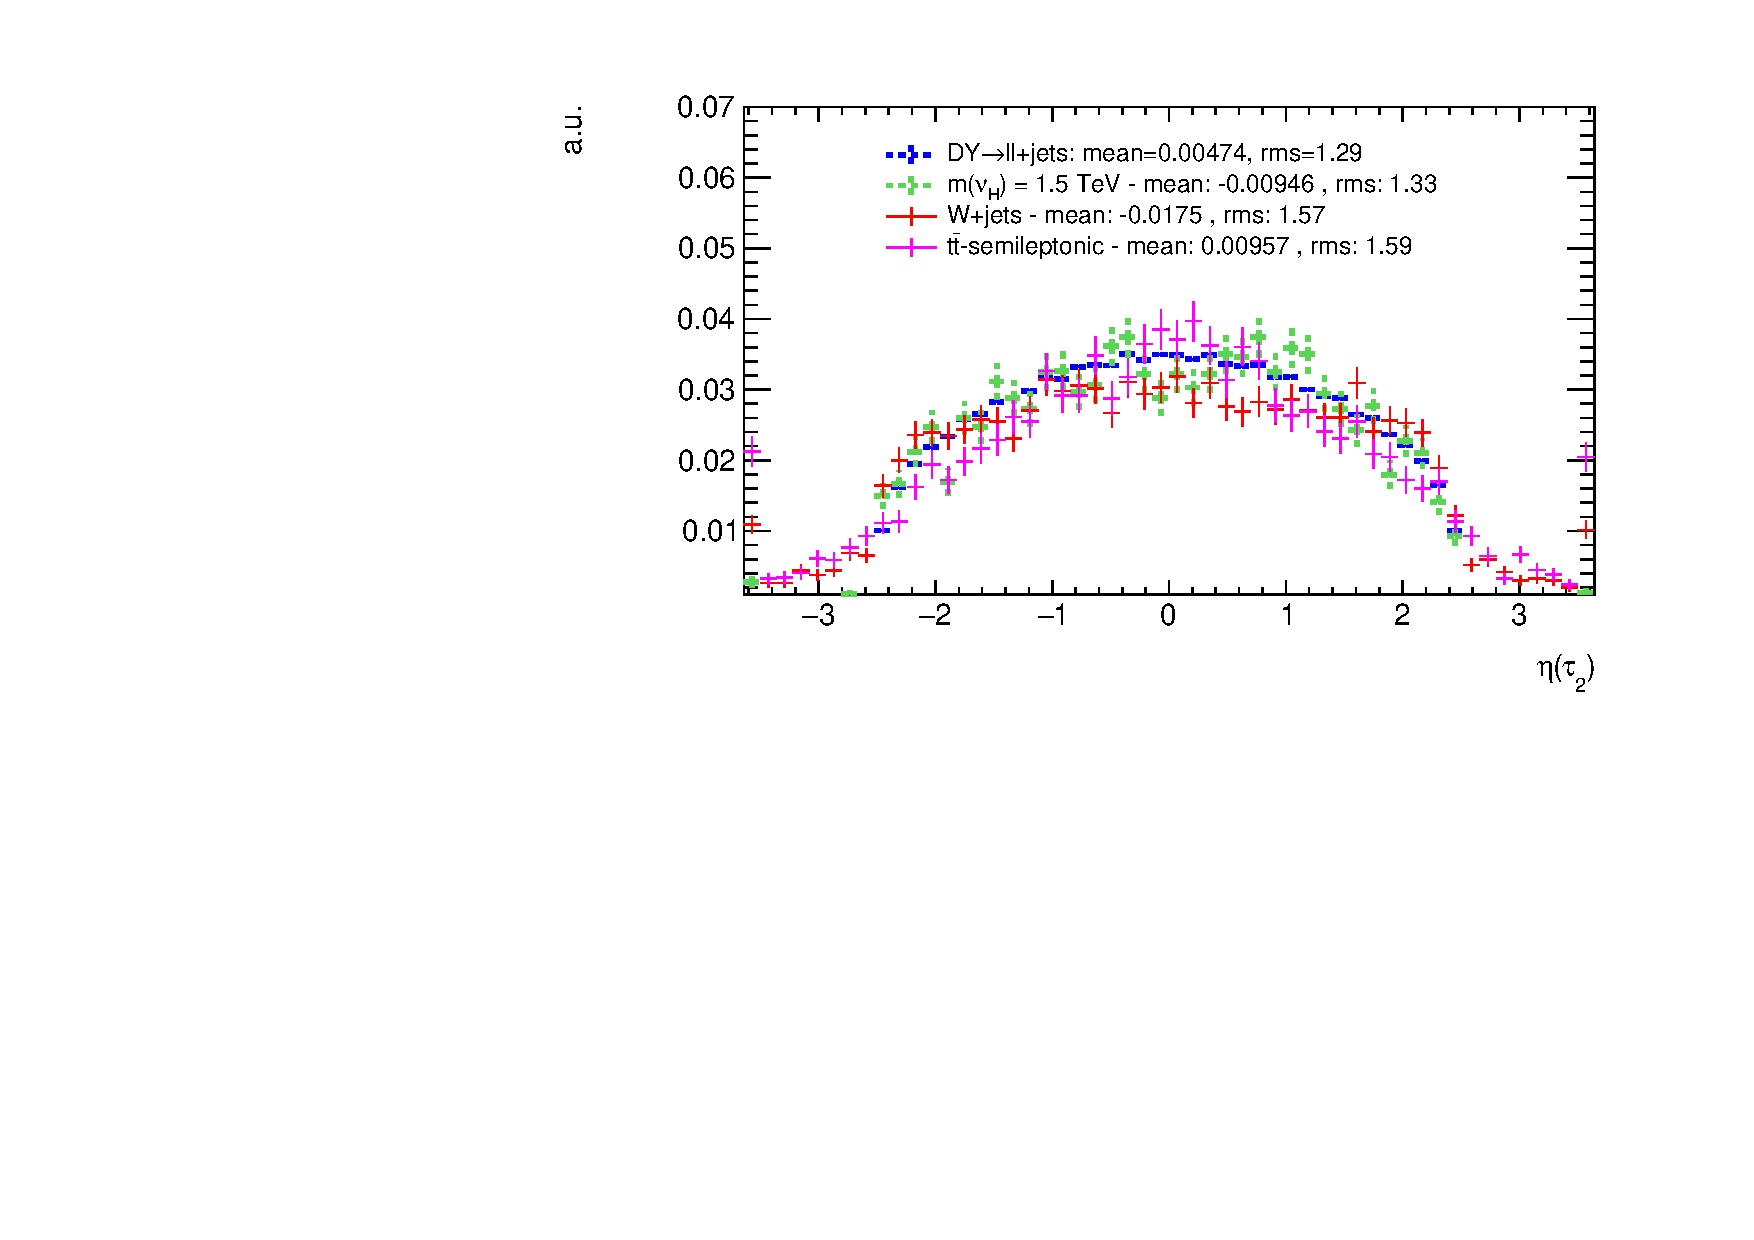
\includegraphics[width=1.2\linewidth]{Figures/Plots/tau2_eta_unitNoCuts.pdf}
\caption{Unit plot of $\eta$ from the sub-leading $\tau$ with no cuts}
\label{fig: tau2etaunitNC}
\end{figure}

\begin{figure}
\centering
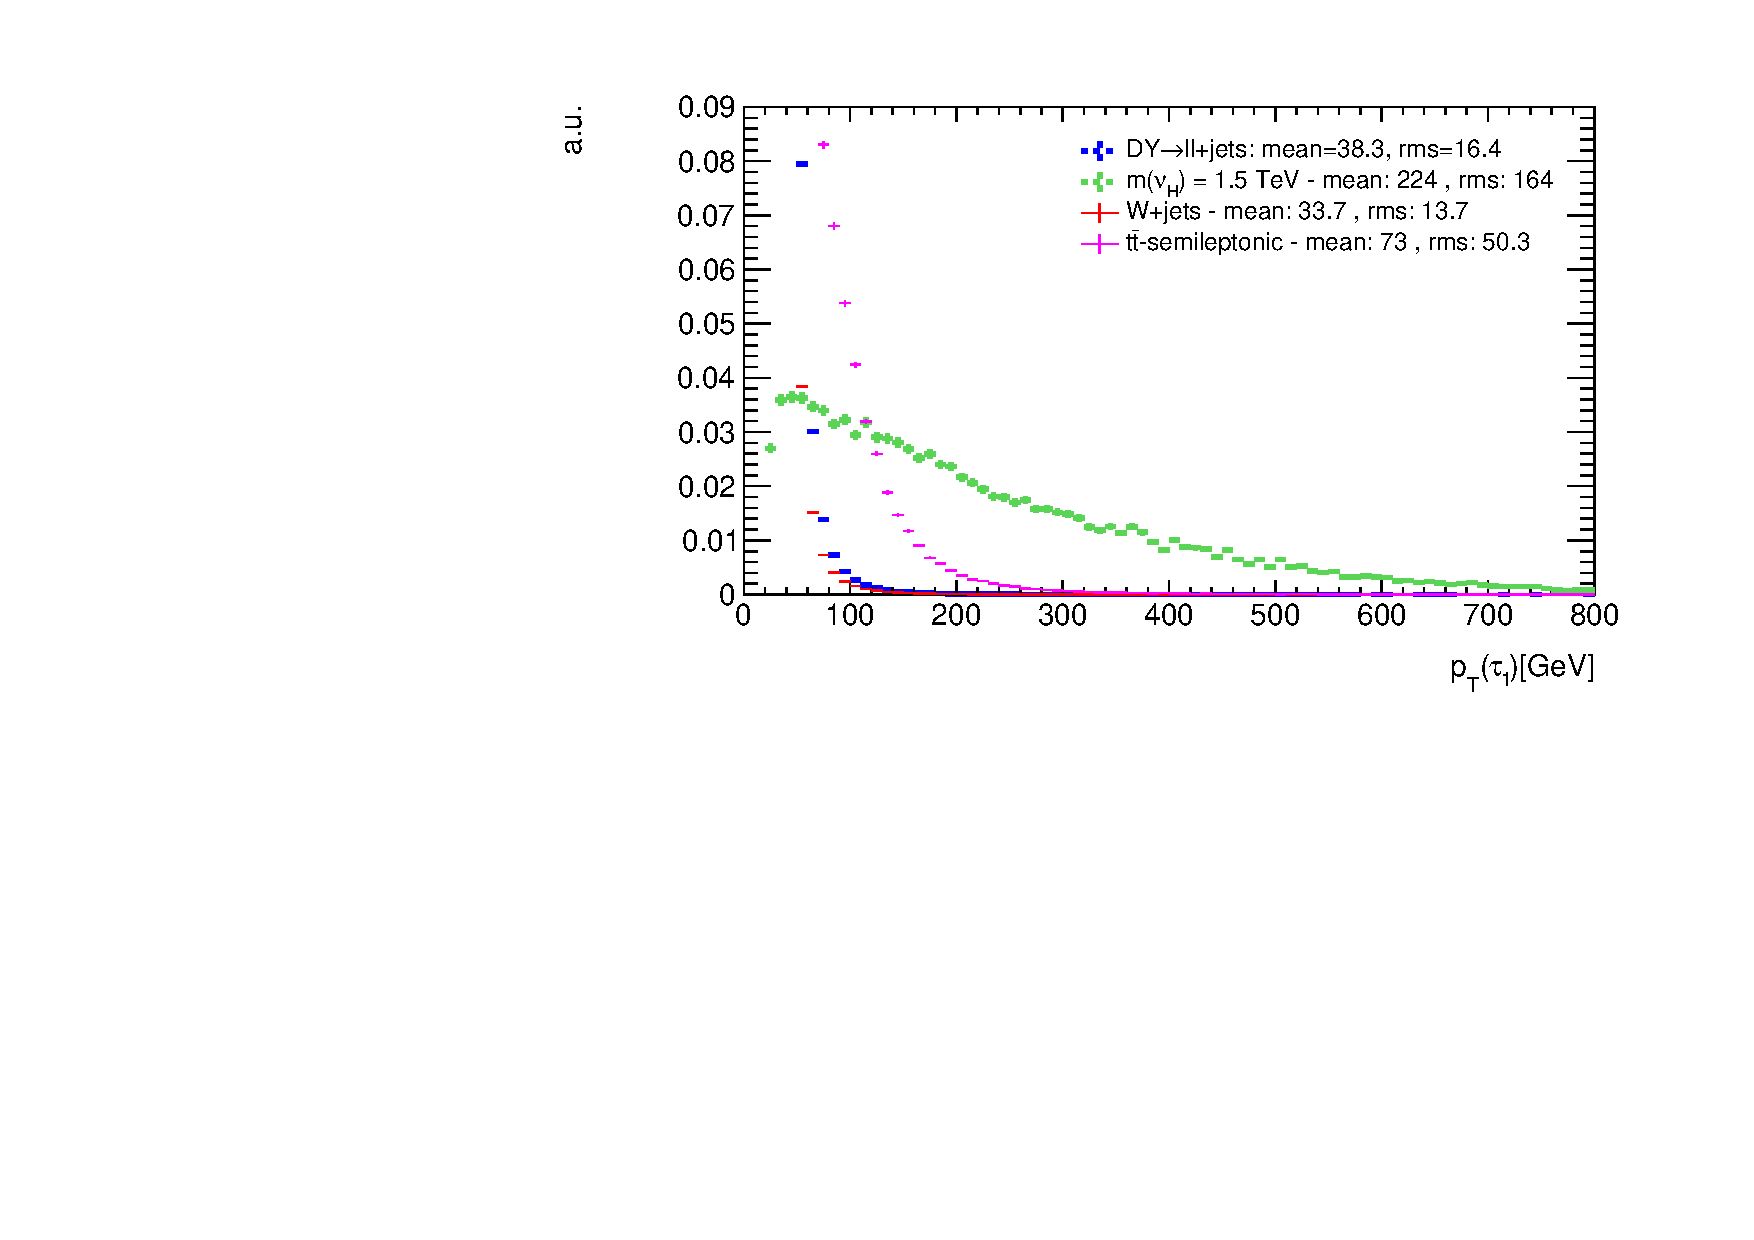
\includegraphics[width=1.2\linewidth]{Figures/Plots/tau1_pt_unitNoCuts.pdf}
\caption{Unit plot of $p_{T}$ of leading $\tau$ with no cuts}
\label{fig: tau1ptunitNC}
\end{figure}

To understand the definition of $H_{T}$ and $S_{T}$ mentioned in chapter \ref{sec:definitions}, the plots in Figure \ref{fig: ptUnitPlots} are shown. The four plots show a separation, in some cases a smaller than others, between the signal and backgrounds distributions. Although the normalized graphics from the jets correspond to the ones of the Di-Jet Pair, that as mentioned in chapter \ref{sec:definitions} were not taken into account in $H_{T}$ and $S_{T}$, a tendency of the signal jets to have greater transverse momentum than the ones in the backgrounds is shown. This tendency is also displayed for both $\tau$'s. Hence, the distributions of $H_{T}$ and $S_{T}$ should show a similar behaviour because this variables are the result of adding the transverse momentum of jets and $\tau$'s in the event.

\begin{figure}       
        \centering
        \begin{subfigure}[b]{0.475\textwidth}
            \centering
            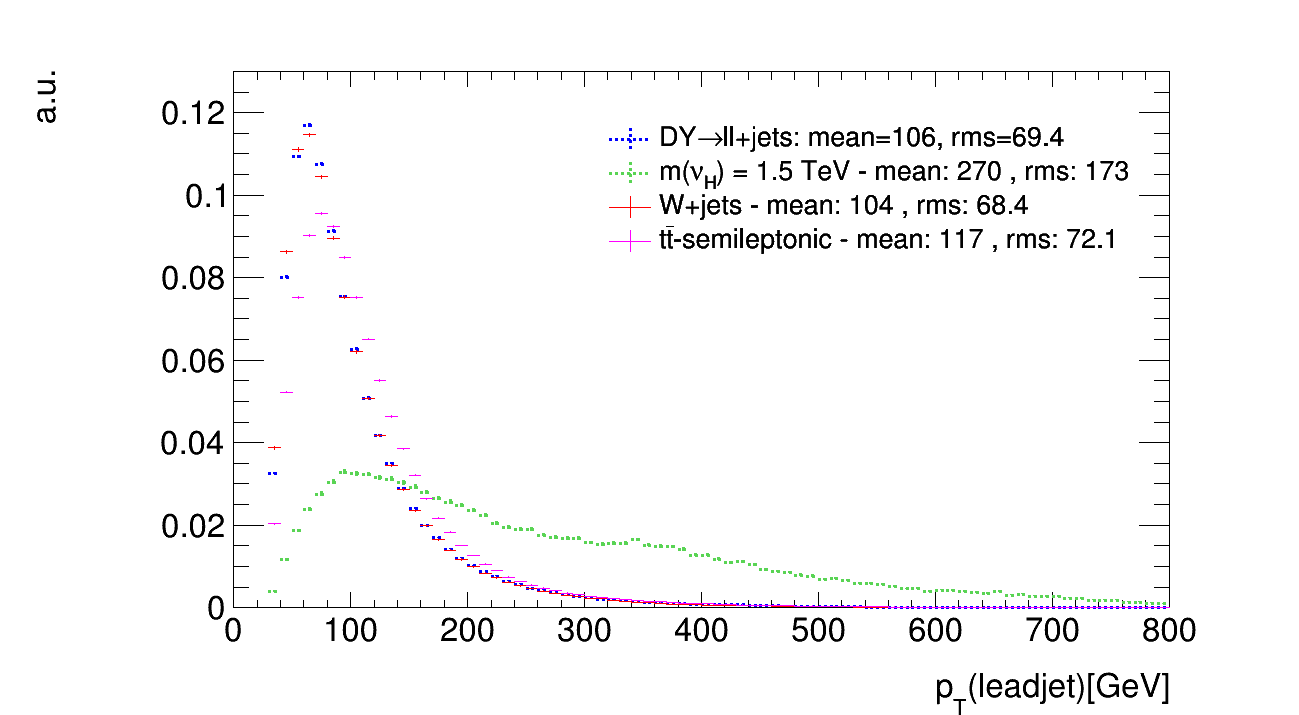
\includegraphics[width=\textwidth]{Figures/Plots/ljet_pt_unitNoCuts}
            \caption[]%
            {{\small Leading jet $p_{T}$ unit plot}}    
            %\label{fig:mean and std of net14}
        \end{subfigure}
        \hfill
        \begin{subfigure}[b]{0.475\textwidth}  
            \centering 
            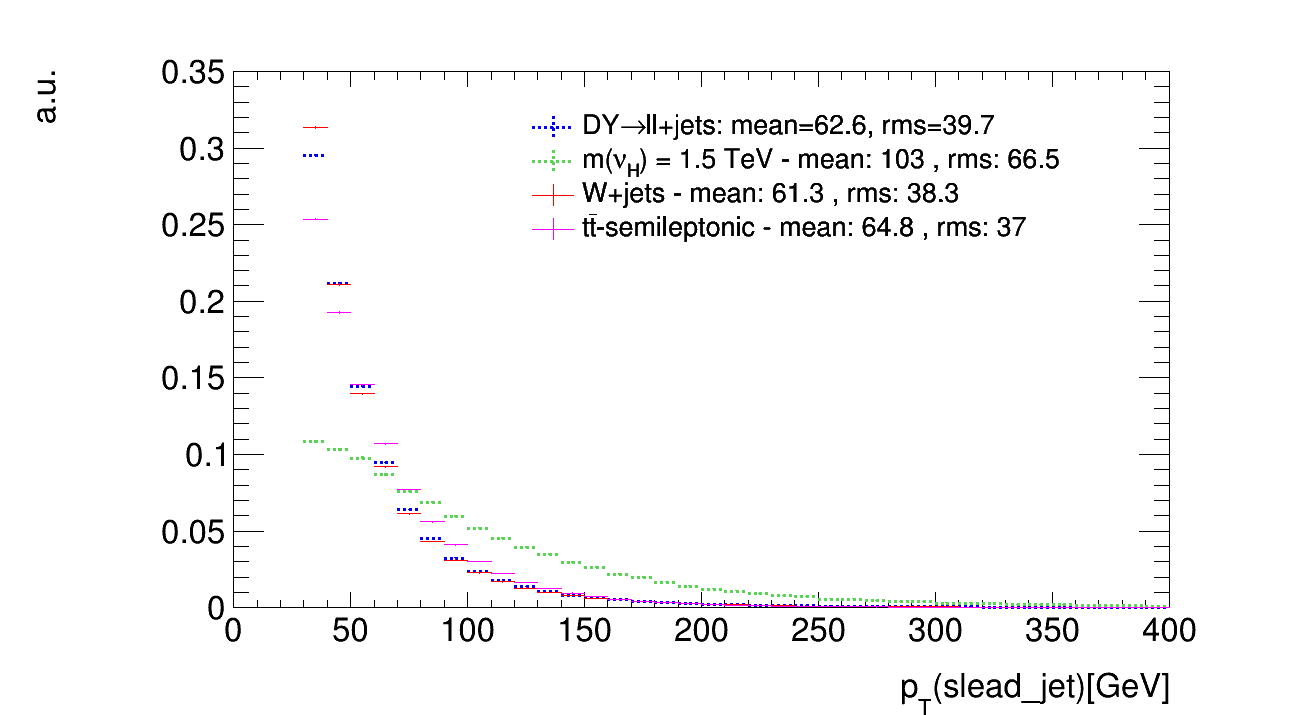
\includegraphics[width=\textwidth]{Figures/Plots/sjet_pt_unitNoCuts}
            \caption[]%
            {{\small Sub-leading jet $p_{T}$ unit plot}}    
            %\label{fig:mean and std of net24}
        \end{subfigure}
        \vskip\baselineskip
        \begin{subfigure}[b]{0.475\textwidth}   
            \centering 
            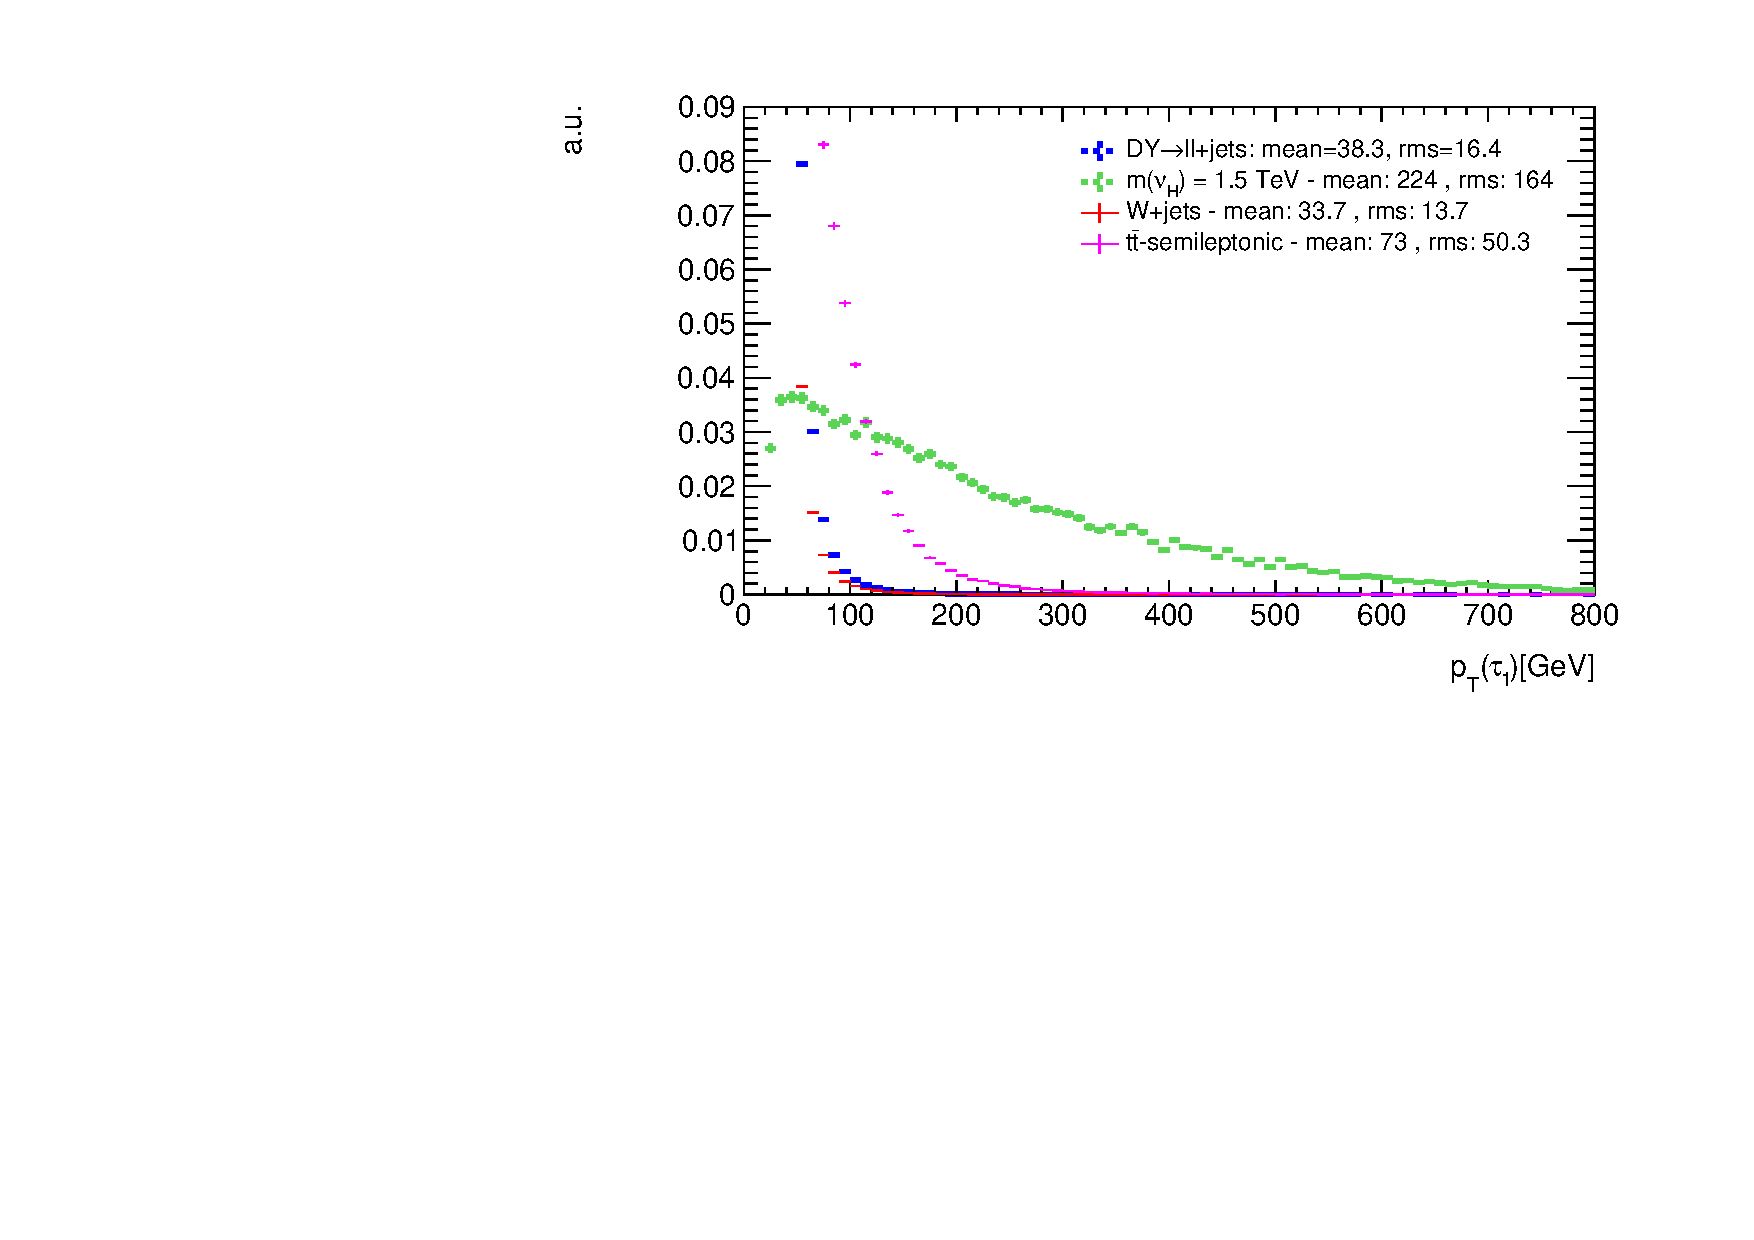
\includegraphics[width=\textwidth]{Figures/Plots/tau1_pt_unitNoCuts}
            \caption[]%
            {{\small Leading $\tau$ $p_{T}$ unit plot}}    
            %\label{fig:mean and std of net34}
        \end{subfigure}
        \quad
        \begin{subfigure}[b]{0.475\textwidth}   
            \centering 
            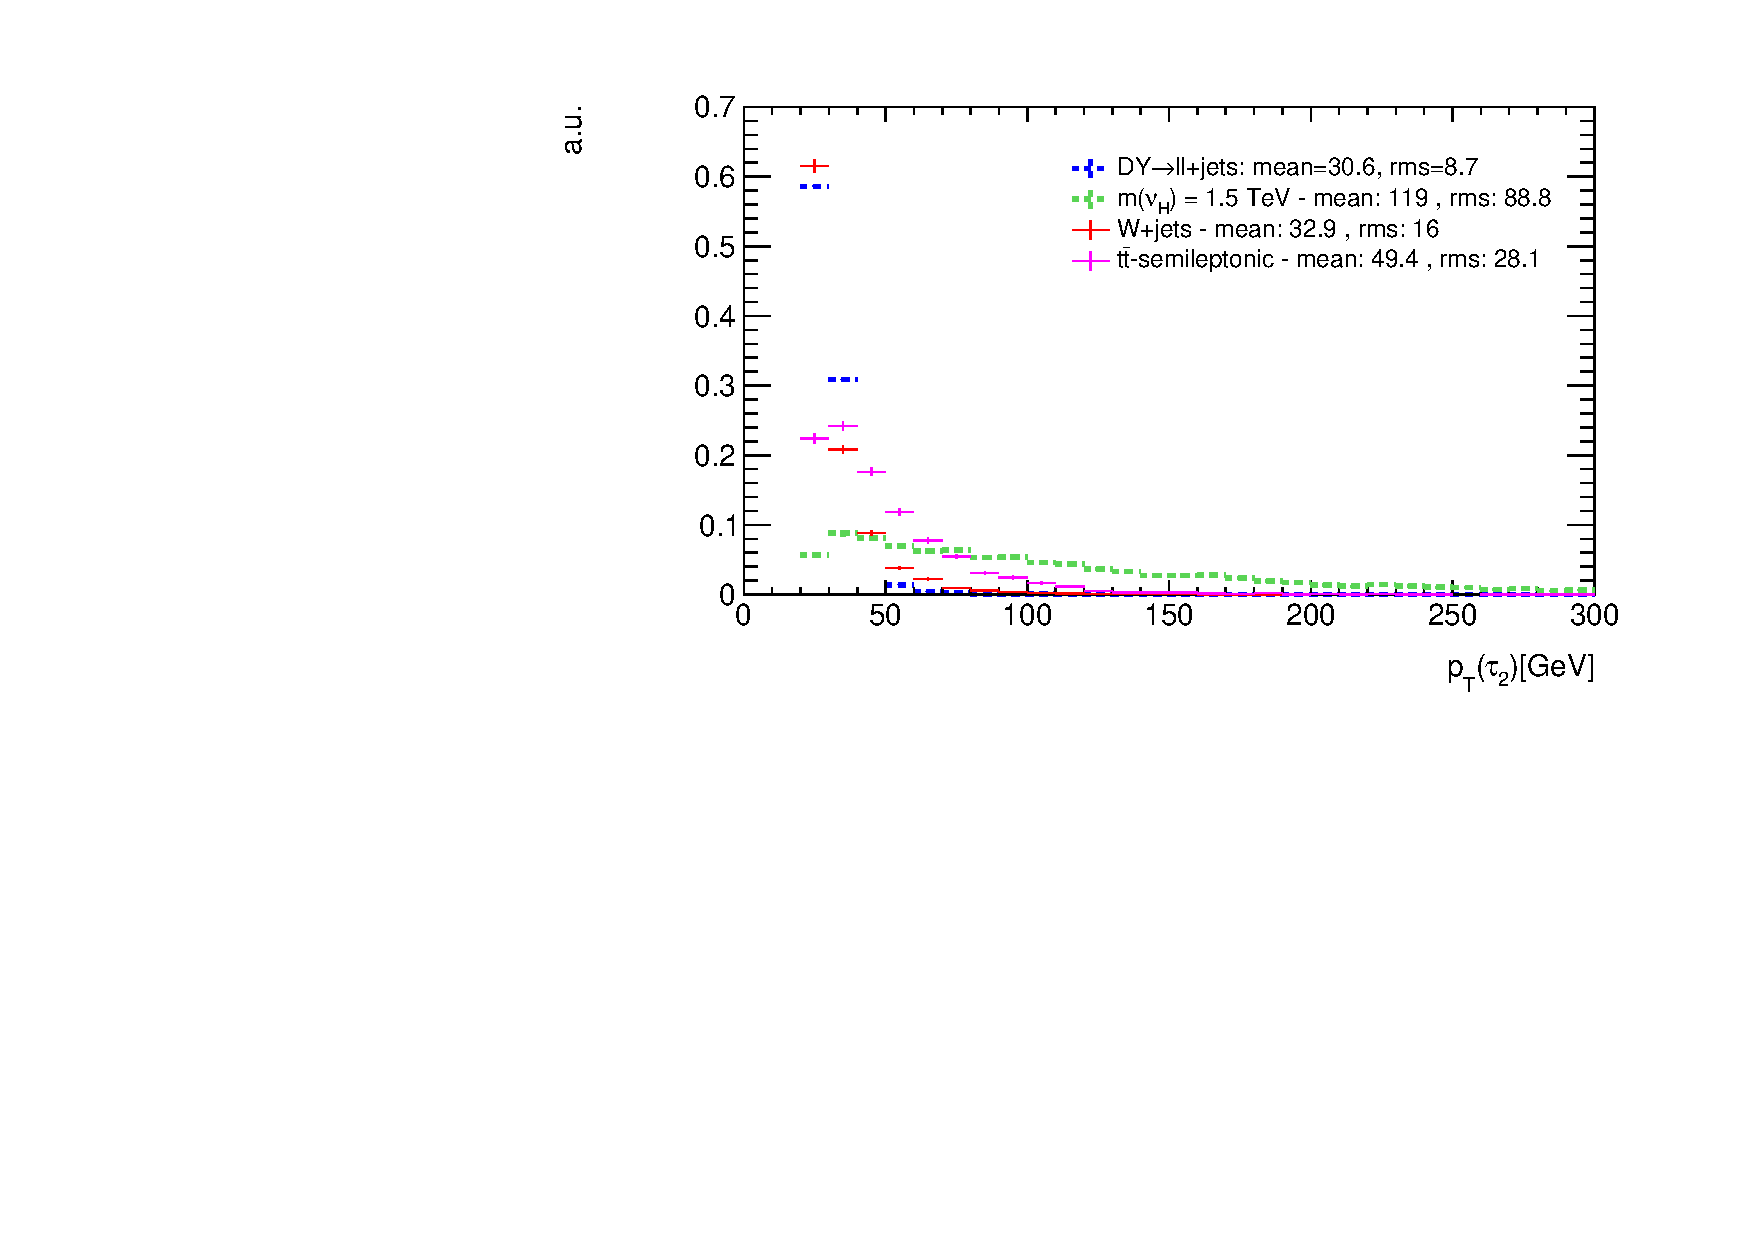
\includegraphics[width=\textwidth]{Figures/Plots/tau2_pt_unitNoCuts}
            \caption[]%
            {{\small Sub-leading $\tau$ $p_{T}$ unit plot}}    
            %\label{fig:mean and std of net44}
        \end{subfigure}
        \caption[ $p_T$ unit plots for different bodies in the event]
        {\small $p_T$ unit plots for different bodies in the event} 
         \label{fig: ptUnitPlots}
\end{figure}

In Figures \ref{fig: HTunitNC} andn \ref{fig: STunitNC}, the normalized plots with no cuts of $H_{T}$ and $S_{T}$ are shown. It can be seen that indeed a greater separation between signal and background was achieved. Unlike the distributions of the $\tau$'s and jets transverse momentum, the maxima of $H_{T}$ and $S_{T}$ lie outside the backgrounds distributions. Furthermore, the background that overlaps at a greater energy with the signal corresponds to $t\bar{t}$. Taking into account what was mentioned in section \ref{sec: cutdefinitions}, the overlap between the signal and this background could be reduced with the cut related with the number of B-jets in the event. This is why this two variables need to be studied closer in the analysis.

\begin{figure}
\centering
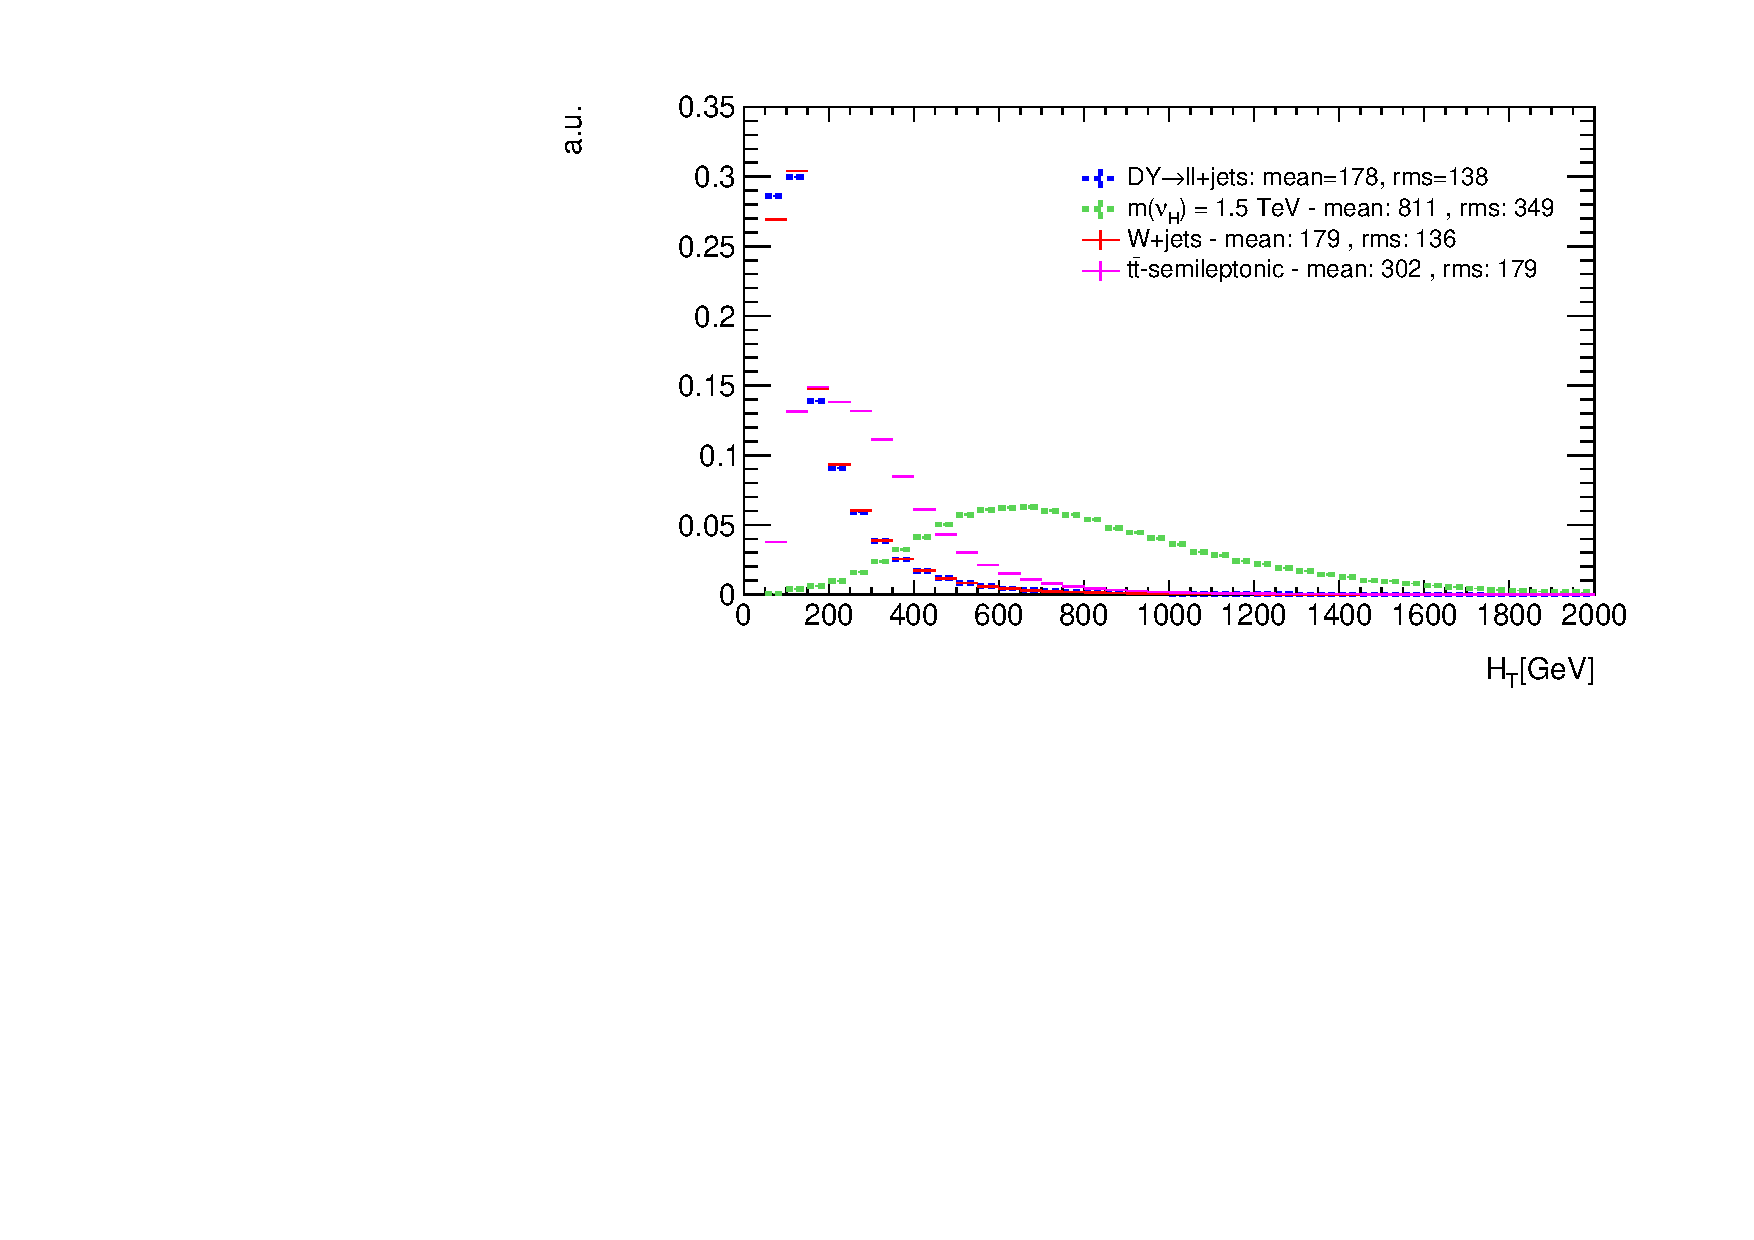
\includegraphics[width=1.2\linewidth]{Figures/Plots/HT_unitNoCuts.pdf}
\caption{Unit plot of $H_{T}$ with no cuts}
\label{fig: HTunitNC}
\end{figure}

\begin{figure}
\centering
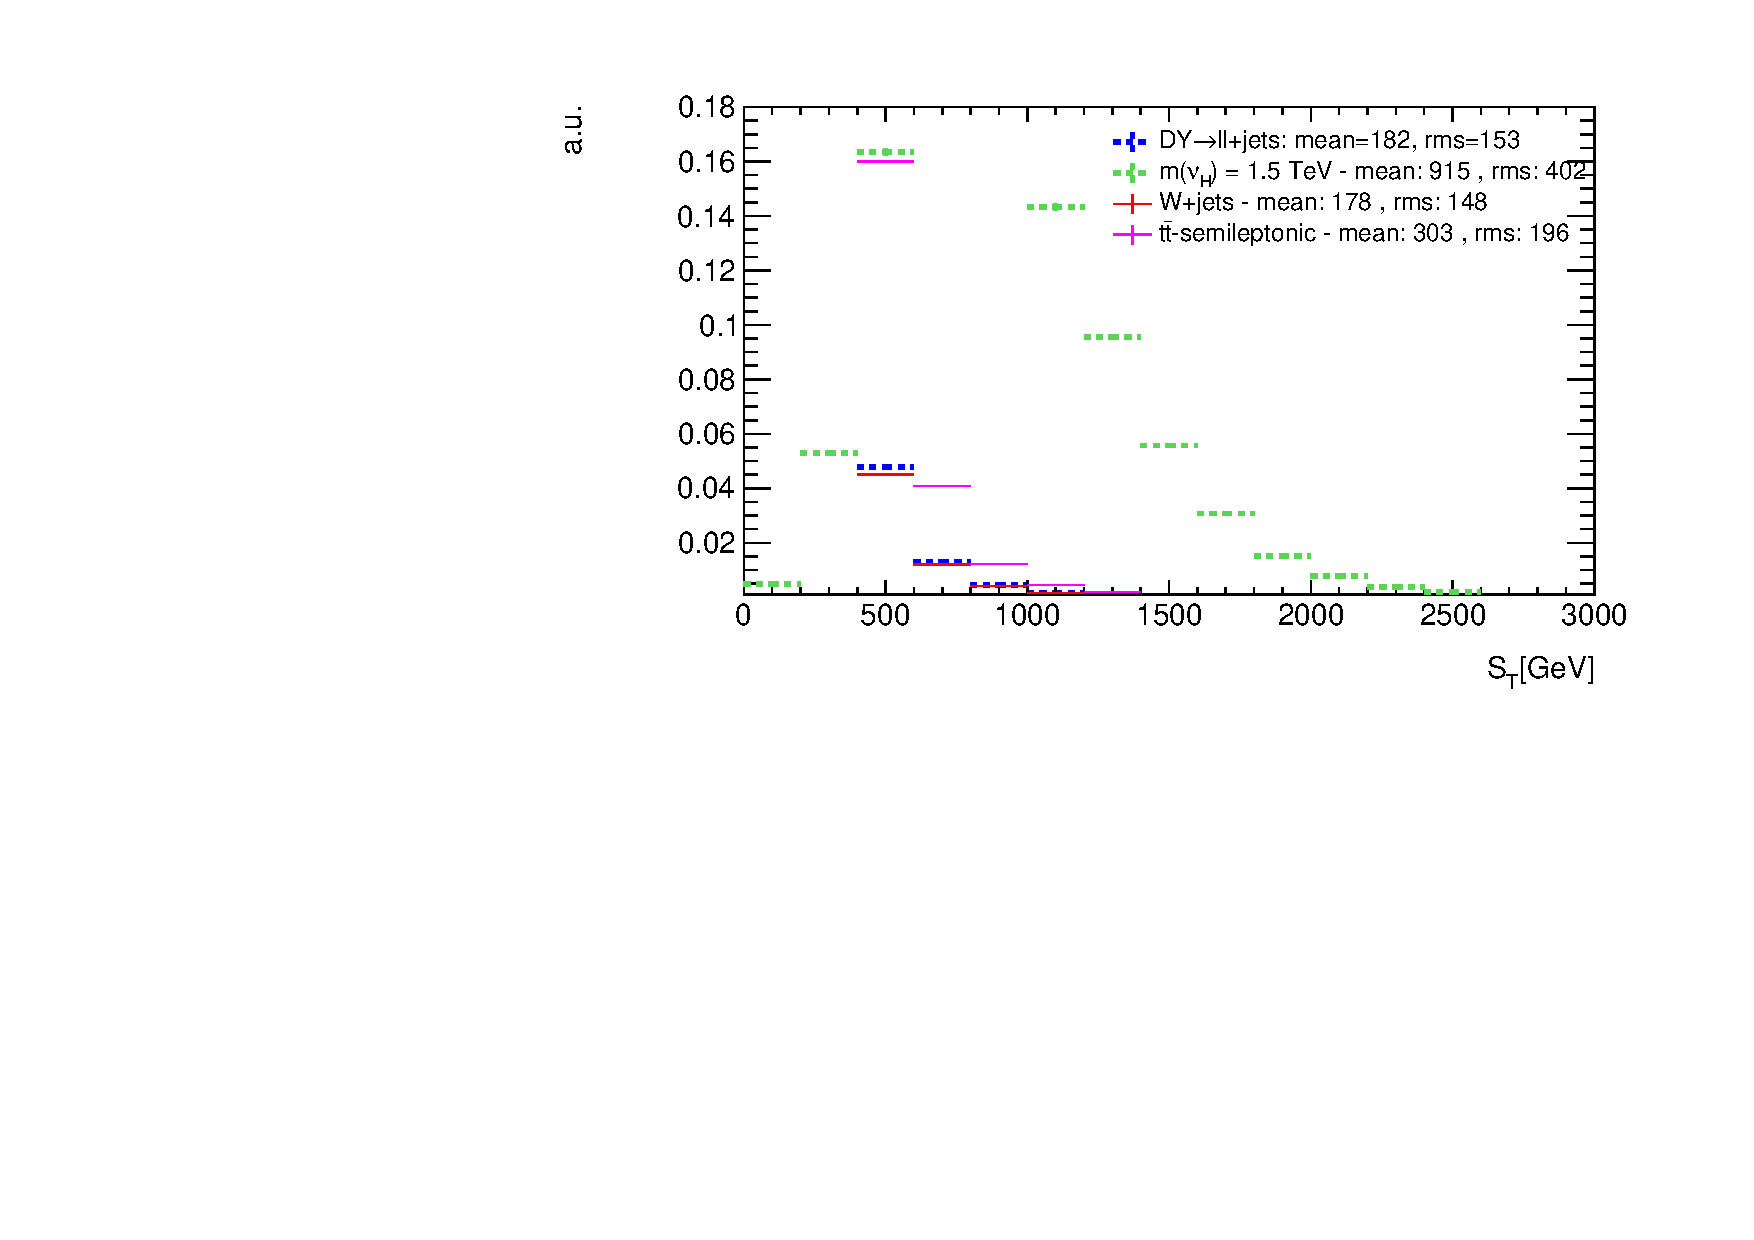
\includegraphics[width=1.2\linewidth]{Figures/Plots/ST_unitNoCuts.pdf}
\caption{Unit plot of $S_{T}$ with no cuts}
\label{fig: STunitNC}
\end{figure}



